\section{Machine Learning}

When looking at artificial intelligence (AI), everything falls on a spectrum from easily explainable to being a black box when thinking about how the machine makes it's decisions.
On the easily explainable side of things, we have things like decision trees.

\begin{figure}[H]
  \centering
  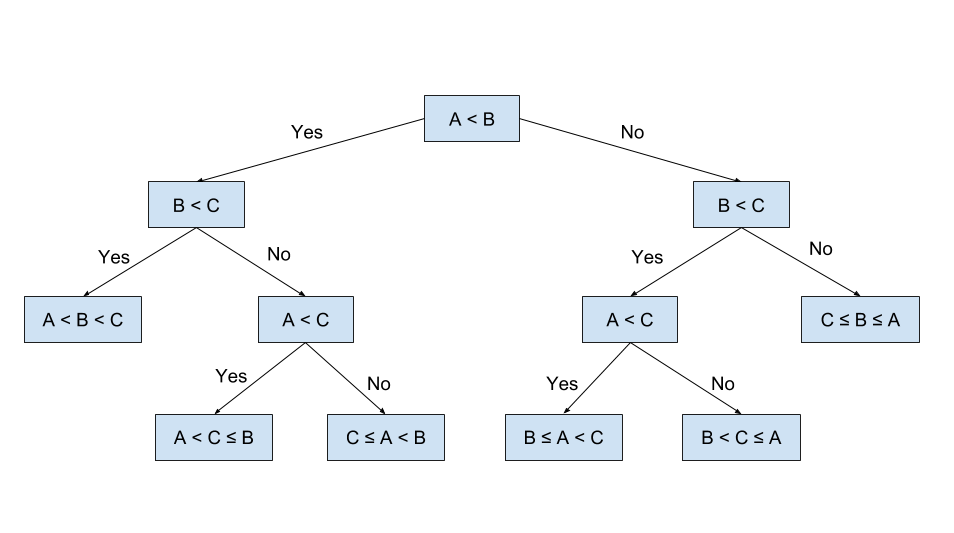
\includegraphics[width=120mm]{figures/decisionTree.png}
  \caption{Example of a basic decision tree}
  \label{decisionTree}
\end{figure}

A decision tree is where we sort the data by asking a sequence of questions and following the flowchart down to where it leads.
By the time we are at the bottom of the tree and have classified the data we can say exactly how the model does it's classification.
For instance if a decision tree is used for mortgage decisions and the model says no, we can query and learn that it said no because you had too low income or too low credit score for instance.

\begin{figure}[H]
  \centering
  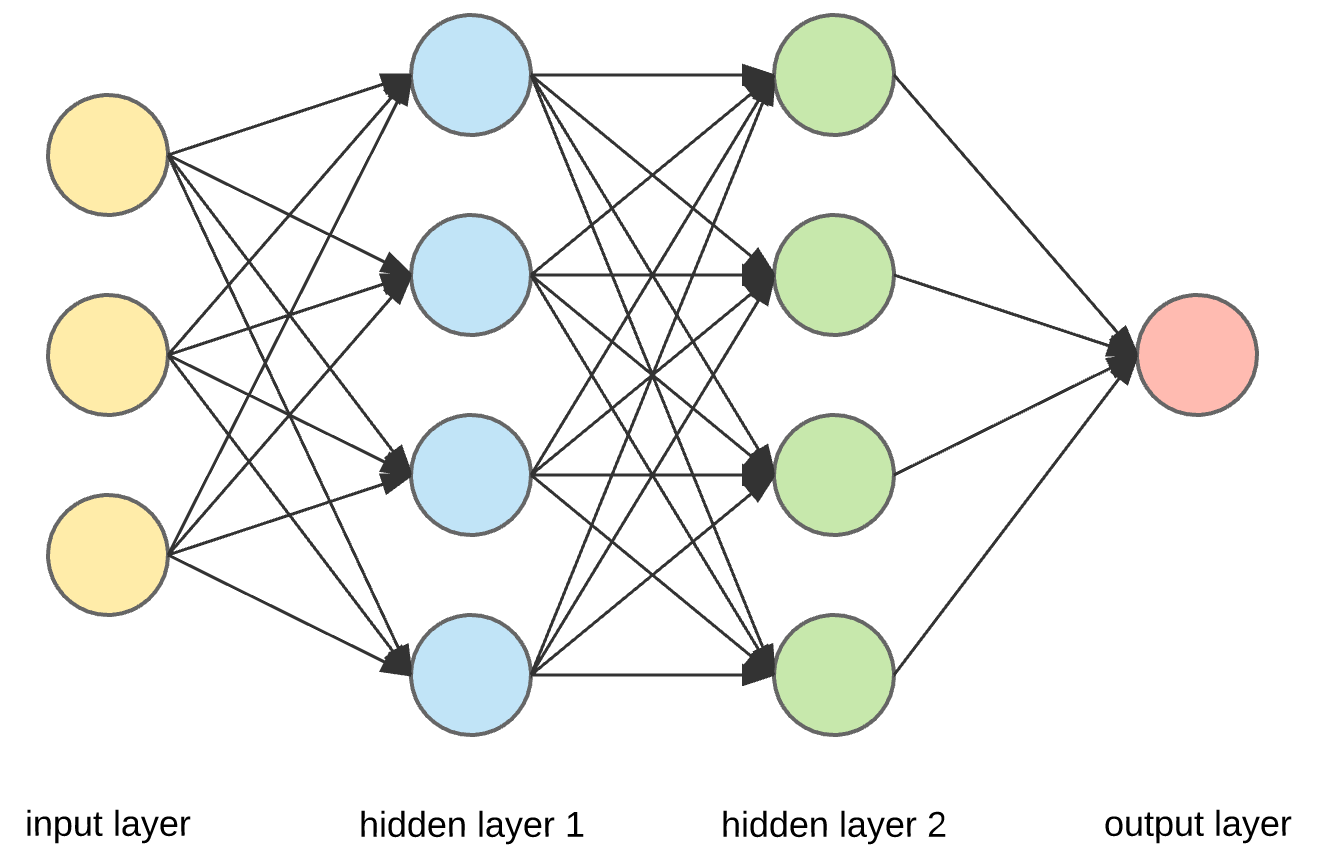
\includegraphics[width=120mm]{figures/neuralNet1.png}
  \caption{Example of a basic Neural Net}
  \label{neuralNet1}
\end{figure}

By contrast, a machine learning model like a neural net is almost a black box with regards to how the decisions are made.
We can query the model and ask it what it made its decisions based on, however, the features it picks out often isn't decipherable to humans in any way.
As in the previous example, if the answer to a mortgage is no, we have no real idea why the model made that decision.
That being said, neural networks are often able to come up with better outcomes for classification that simple models like decision trees are.
In the mortgage example, even if the neural net can't tell us how it comes to the conclusion of approving a loan, it is still more likely to be able to better tell who will be a good credit risk compared to the decision tree.
That's often the trade off that we make when deciding on a more opaque model.
That's why even though they are opaque in how they come up with their answers we still rely on them so heavily.
Because we can empirically test through monte-carlo studies how well they perform both in term of efficiency as well as how often these models misidentify the data that we are throwing at it.

While a neural network is opaque about how the decisions are made, the model itself doesn't have to be a black box for us.
We can take a peek under the hood and see how these models work.
To do so, we start up from the basic models like a perceptron and work our way to a graph neural network, finally connecting it to how neutrino reconstruction works.

\subsection{Perceptron Neuron}

A lot of things that seem incredibly easy to humans -- such as  recognizing the difference between say a cat and a dog -- are very difficult for computers to do.
What makes it difficult to make that sort of classification is that it is hard for humans to define concrete rules about what makes the picture of a cat different than the picture of a dog.
Neural nets approach this in a completely different fashion.

Instead of trying to define rules about the features that differentiate the picture of a dog vs a cat, we instead classify a whole bunch of pictures by hand.
\footnote{This is true only for supervised learning.
Unsupervised learning doesn't require classification by hand but have their own set of disadvantages}
Then throw those pictures at the algorithm with the correct answers and over time the computer learns to tell the difference between that of a dog and a cat.
We call an algorithm like this that separates things into two piles a binary classifier.
There are many different kinds of binary classifiers with a whole host of advantages and disadvantages but we will start with one that is simple to understand; the perceptron.

\begin{figure}[H]
  \centering
  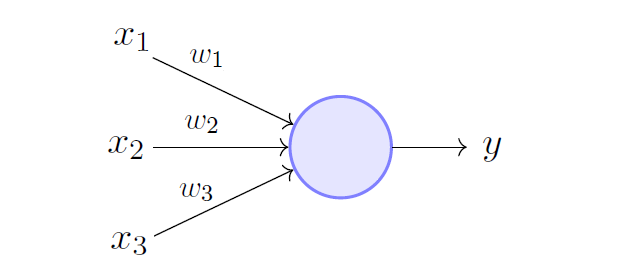
\includegraphics[width=120mm]{figures/perceptron1.png}
  \caption{Perceptron Neuron \cite{El-Amir_Hamdy_2019}}
  \label{perceptron1}
\end{figure}

A perceptron takes a number of inputs that are binary in nature and produce a single binary output \cite{Freund_Schapire_1998} ie.is this a dog? The figure \ref{perceptron1} has 3 inputs ($x_1$, $x_2$ and $x_3$) although, more or fewer inputs may be used.
Each input then is given a weight -- $w_1$, $w_2$ and $w_3$ in this case -- and the output calculated thus.

\begin{align}
  y = \begin{cases}
    0 \textrm{ if } \sum_i w_i x_i \leq \textrm{threshhold},\\
    1 \textrm{ if } \sum_i w_i x_i > \textrm{threshhold},\\
  \end{cases}
\end{align}

Used in this fashion, a perceptron can only make simple choices.
Raising the threshold makes the classification tighter while lowering it loosens the classification.
Because the output of a perceptron is binary, for more subtle distinctions, we can use the output of a perceptron to feed into the input of the next one thus creating a network that is more able to measure subtlety.

\begin{figure}[H]
  \centering
  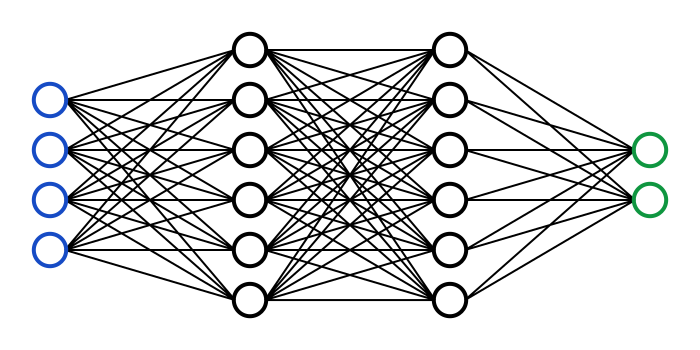
\includegraphics[width=120mm]{figures/network.png}
  \caption{Perceptron network \cite{Zhou_2020}}
  \label{network}
\end{figure}

Varying the weights of the inputs in combination with the threshold for the output allows us to get different models of classification.
The neurons in the first layer are only able to make simple decisions based on the raw input but because we use their output as the input to the second layer, the second layer can make more abstract decisions with a degree of subtlety impossible not only with one perceptron but also with even a single layer of perceptrons.
The complexity of the discrimination by the classifier increasing with both the number and layers of perceptrons in the network.

With the correct weights and threshold values, we can get any binary classifier we want using a set of perceptrons.
That, however, puts us back at our original problem of classifying whether something is a dog; namely, if we knew what features to look for (i.e.\ what weights and threshold to use) it wouldn't be hard explaining to a computer what a dog was.
The true innovation comes with using learning algorithms that don't require input from the programmer to set these weights and thresholds.

  If we want to use algorithms that can adjust weights and thresholds (otherwise called biases) automatically, we need some method where a small change in the weight only causes a small change in the output.
Because perceptrons are binary, this is impossible to do with only perceptrons.

  A small change in the weight to an input to the perceptron can flip the output entirely.
While this small change in weight can make one of the outputs of the network better, it may also affect the rest of the network behave in unpredictable ways.
Going back to the dog and cat example, while changing the weight slightly may make it better at recognizing dogs, it may wreak havoc on how cats are identified.

  This is where sigmoid neurons come in.

\subsection{Sigmoid Neuron}

While perceptrons are effectively step functions, flipping from $0$ to $1$, sigmoids are more smoothed out.
This means that a small change in the weight can lead to a small change in output\cite{Nielson_2020}.
The sigmoid function can be written as

\begin{align}
  \sigma = \frac{1}{1 + e^{-z}}
\end{align}

This means that a sigmoid neuron can be written as

\begin{align}
  \frac{1}{1 + e^{-\sum_i w_i x_i - b}}
\end{align}

where the $b$ stands for the bias of every input.
While this looks different than the perceptron at first glance it is just a more smoothed out version of it.
One key thing that we lose with the introduction of sigmoids is the linearity that perceptrons afforded us.
What we gain is the ability for our programs to automatically adjust their weights and biases because a small change in weights does lead to small change in output as shown in equation \ref{bias}.

\begin{align}\label{bias}
  \Delta y \approx \sum_i \frac{\partial y}{\partial w_i}\Delta w_i + \frac{\partial y}{\partial b}\Delta b
\end{align}

\begin{figure}[H]
  % https://blog.roboflow.com/activation-function-computer-vision/
  \centering
  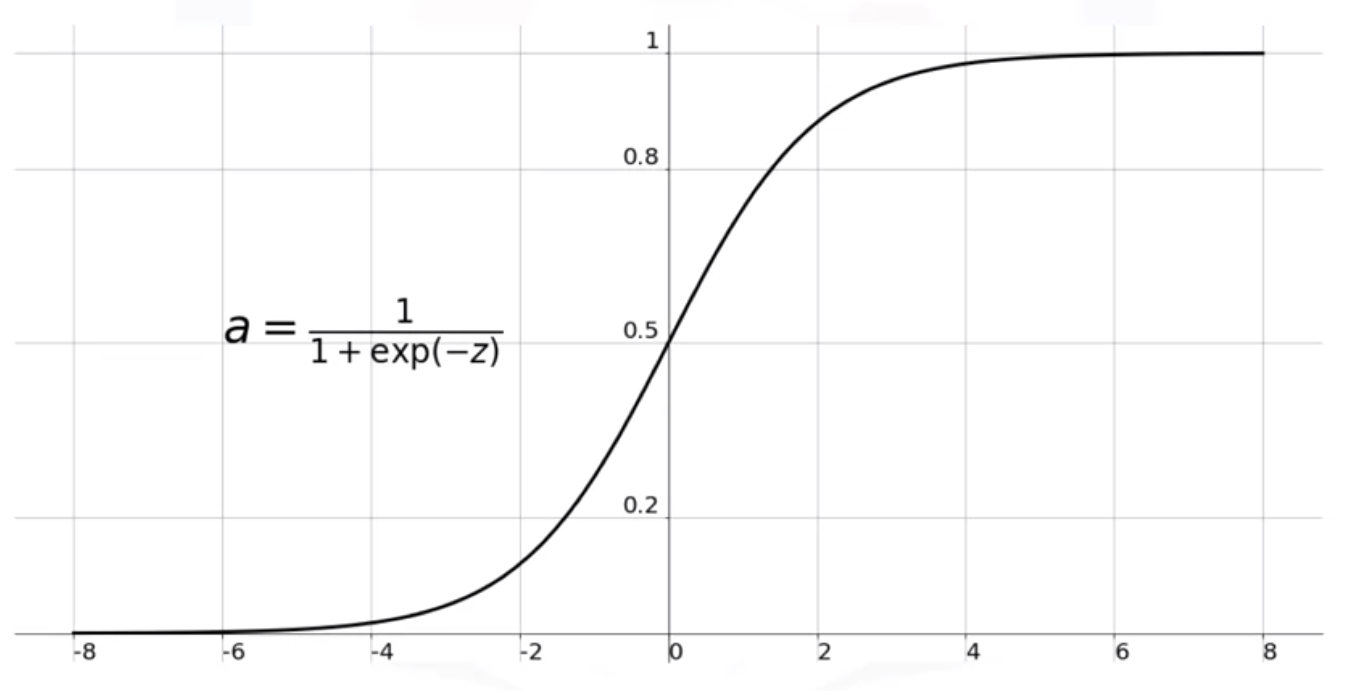
\includegraphics[width=80mm]{figures/sigmoid.png}
  \caption{Sigmoid Function \cite{Potrimba_2023}}
  \label{network}
\end{figure}

More than the exact formula of the sigmoid neuron what matters is the shape.
As a result, other neurons can be used in its stead which retain the property of having a small change in weight lead to a small change in output.
Some of the more popular of these functions (called activation functions) are RELU and softmax.
Each have their own advantages and disadvantages and may even be mixed in the same neural network



\subsection{Activation Functions}

One drawback of the sigmoid function is that its gradients can become very small for large positive or negative inputs, leading to the vanishing gradient problem during backpropagation.
Backpropagation is an optimization algorithm used to minimize the error of neural networks by calculating the gradient of the loss function with respect to each weight through the chain rule and updating the weights accordingly\cite{KELLEY_1960} \cite{Bryson_1962} .

The hyperbolic tangent function is another activation function that provides output values between -1 and 1.
It is defined as:

\begin{align}
  \tanh(z) = \frac{e^z - e^{-z}}{e^z + e^{-z}}
\end{align}

\begin{figure}[H]
  % 
  \centering
  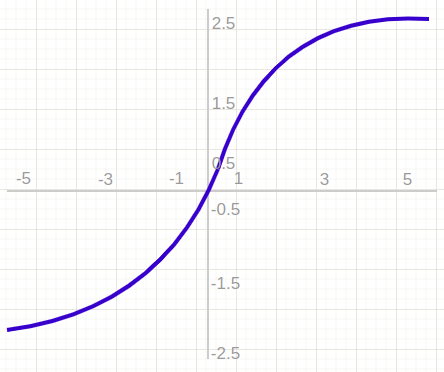
\includegraphics[width=80mm]{figures/tanh.png}
  \caption{tanh Function \cite{Potrimba_2023}}
  \label{tanh}
\end{figure}

In a neural network, a neuron with the tanh activation function computes:

\begin{align}
  \tanh(\sum_i w_i x_i + b) = \frac{e^{(\sum_i w_i x_i + b)} - e^{-(\sum_i w_i x_i + b)}}{e^{(\sum_i w_i x_i + b)} + e^{-(\sum_i w_i x_i + b)}}
\end{align}

The tanh function is zero-centered, which helps in making the learning process faster and more efficient compared to the sigmoid function.
It also suffers from the vanishing gradient problem, though it generally performs better in practice than sigmoid.

The Rectified Linear Unit (ReLU) is a widely used activation function in deep learning models.
It is defined as:

\begin{align}
  \text{ReLU}(z) = \max(0, z)
\end{align}

\begin{figure}[H]
  % 
  \centering
  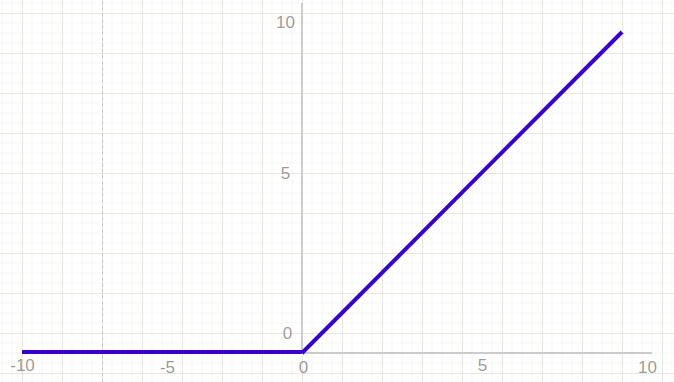
\includegraphics[width=80mm]{figures/relu.png}
  \caption{RELU function \cite{Potrimba_2023}}
  \label{relu}
\end{figure}

For a neuron using ReLU, the output is computed as:

\begin{align}
  \text{ReLU}(\sum_i w_i x_i + b) = \max(0, \sum_i w_i x_i + b)
\end{align}

ReLU introduces non-linearity while being computationally efficient.
It helps mitigate the vanishing gradient problem by allowing gradients to flow more easily through the network\cite{Goodfellow_2016}.
However, it suffers from the "dying ReLU" problem where neurons can sometimes become inactive and only output zero.

To address the dying ReLU problem, the Leaky ReLU function introduces a small, non-zero gradient for negative inputs \cite{Maas_Hannun_Ng_2014}.
It is defined as:

\begin{align}
  \text{Leaky ReLU}(z) = \begin{cases}
    z & \text{if } z > 0 \\
    \alpha z & \text{if } z \leq 0
  \end{cases}
\end{align}

where \( \alpha \) is a small constant (e.g., 0.01).

\begin{figure}[H]
  % 
  \centering
  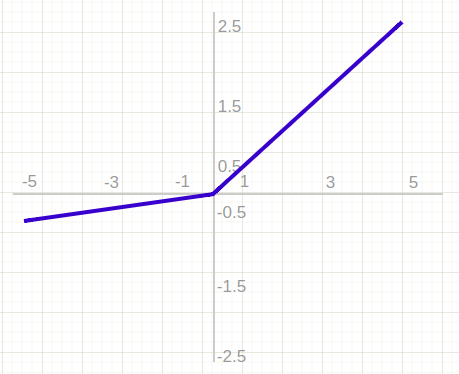
\includegraphics[width=80mm]{figures/lrelu.png}
  \caption{Leaky RELU function \cite{Potrimba_2023}}
  \label{lrelu}
\end{figure}
For a neuron using Leaky ReLU, the output is:

\begin{align}
  \text{Leaky ReLU}(\sum_i w_i x_i + b) = \begin{cases}
    \sum_i w_i x_i + b & \text{if } \sum_i w_i x_i + b > 0 \\
    \alpha (\sum_i w_i x_i + b) & \text{if } \sum_i w_i x_i + b \leq 0
  \end{cases}
\end{align}

The Exponential Linear Unit (ELU) is designed to combine the benefits of ReLU and Leaky ReLU while addressing their limitations.
It is defined as:

\begin{align}
  \text{ELU}(z) = \begin{cases}
    z & \text{if } z > 0 \\
    \alpha (e^z - 1) & \text{if } z \leq 0
  \end{cases}
\end{align}

where \( \alpha \) is a positive constant.

\begin{figure}[H]
  % Different Cite
  % https://www.researchgate.net/figure/The-exponential-linear-unit-ELU-activation-function_fig3_350283420
  \centering
  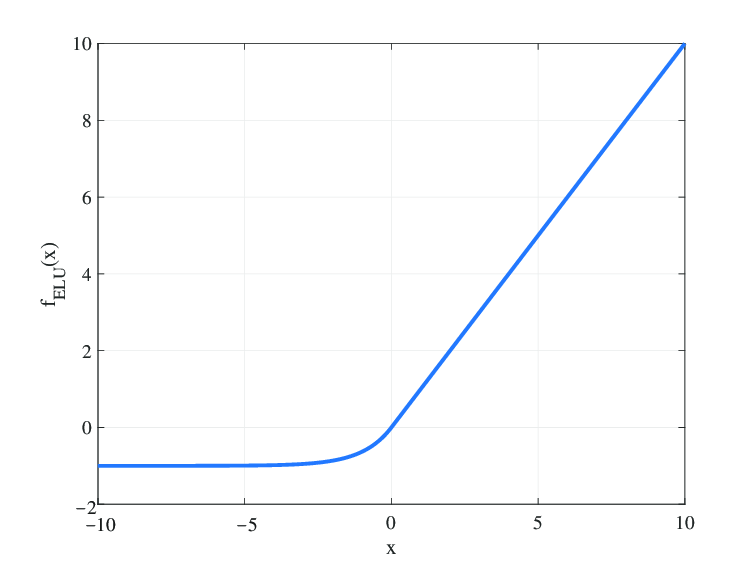
\includegraphics[width=80mm]{figures/elu.png}
  \caption{ELU function \cite{Sheng_2021}}
  \label{elu}
\end{figure}
For a neuron using ELU, the output is:

\begin{align}
  \text{ELU}(\sum_i w_i x_i + b) = \begin{cases}
    \sum_i w_i x_i + b & \text{if } \sum_i w_i x_i + b > 0 \\
    \alpha (e^{(\sum_i w_i x_i + b)} - 1) & \text{if } \sum_i w_i x_i + b \leq 0
  \end{cases}
\end{align}

ELU can help speed up learning and improve robustness to noise by reducing the impact of vanishing gradients.



\subsection{Neural Network}

A number of these sigmoid neurons (or neurons with other activation functions) can be strung together to make a neural network.
Each neural network has 3 main parts.

\begin{figure}[H]
  \centering
  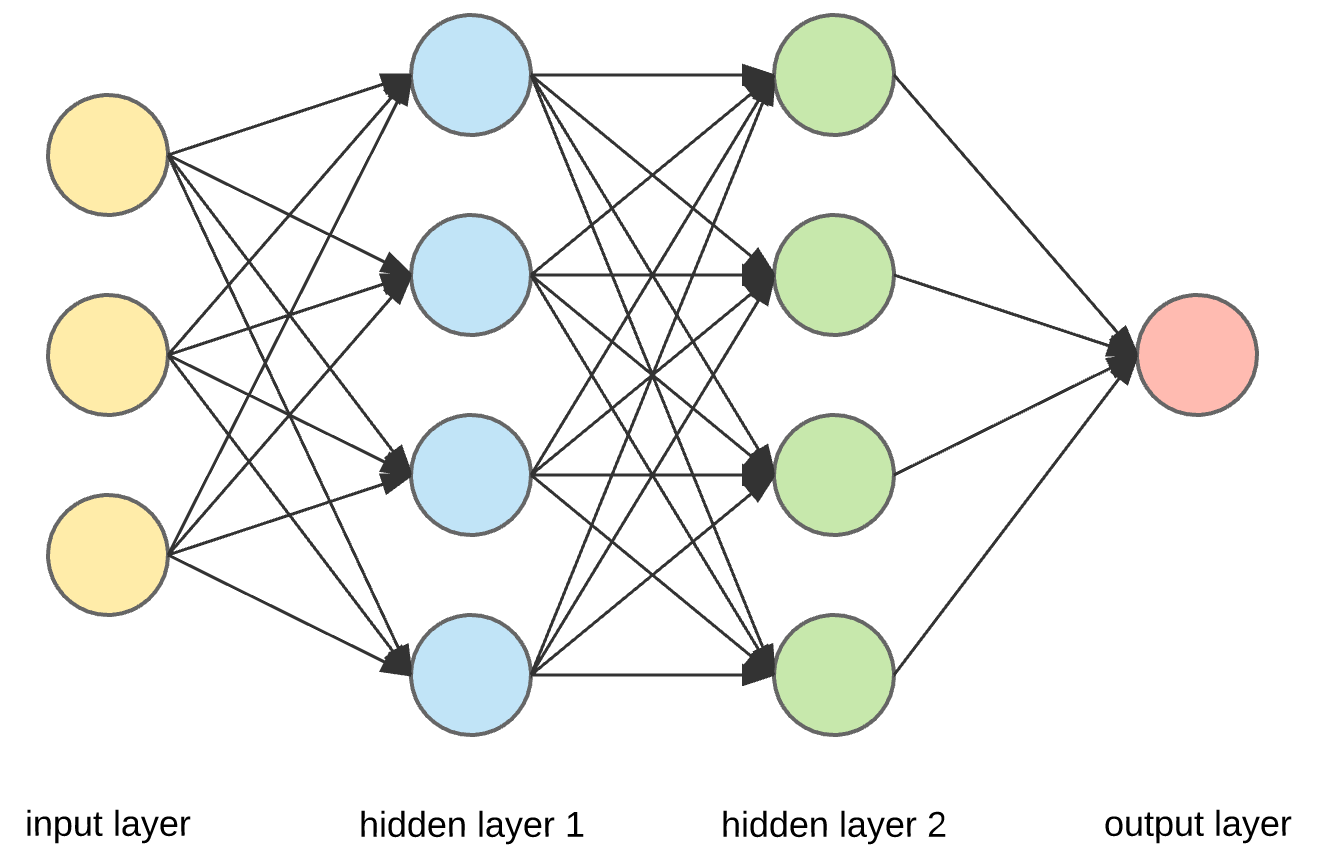
\includegraphics[width=120mm]{figures/neuralNet1.png}
  \caption{Parts of a Neural Net}
  \label{neuralNet2}
\end{figure}

First, we have an input layer.
This is all the inputs that go into a neural network and is usually represented as a vector.
Each input adds one to the dimension of the input vector.
Even something like a 2d picture can have its rows stitched together to make one long vector of inputs.

The middle bits are called the hidden layer, not for any profound reason, but just to distinguish them from the input and output layers.
You can have as many hidden middle layers as you want in the network.
The trade off is usually one of efficiency and accuracy.
The more hidden layers you have, the more accurate the output will bebut at the cost of requiring more time to train because there are more weights to get right.
After a point, adding more layers does not improve accuracy in meaningful way while still taking longer to train.
This makes creating a good neural net less of a hard science and more of an art form.

Finally, we have the output layer.
This layer usually has one neuron for each thing the classifier can bin the input into.
In the dog and cat case, we would have $2$ output neurons, one that signifies dog and the other cat.
However, the neurons won't directly tell us whether the picture contains a dog or a cat but rather give us two values.
One of these values indicates how likely it is for this picture to contain a cat and the other represents the likelyhood that the picture contains a dog.
After that, it is still up to us to decide on cutoff values to determine whether we will say the picture contains a cat, a dog, both or neither.


\subsection{Gradient Descent}

So far we've talked about the fact that weights and biases can be adjusted and that it only works if a small change creates only a small change in output while glossing over how exactly the computer automatically calculates these weights.
Time to peel back that layer!
\footnote{pun very much intended}
We use a technique called gradient descent.

To start off, we need a set of inputs $x$ where we already know the answers $y$.
This is called the training dataset.
Once the weights and biases are adjusted we can then use the model to query a set of inputs that we don't know and be reasonably certain that it won't give us garbage outputs.
To do this adjustment, we need to define a cost function.

\begin{align}
  C(w,b) = \frac{1}{2n} \sum_x || y(x) - a||^2
\end{align}

Where $n$ is the number of training samples and $a$ is the vector of outputs from the network.
We want a set of weights that make the cost as small as possible and we can do that through a method called gradient descent.
The function described here is not the only cost function possible but is a simple one to start with.
To use gradient descent, we can do

\begin{align}
  \Delta v = - \eta \nabla C
\end{align}

where $v$ is the set of weights and biases and $\eta$ is the learning rate.
The more aggressive we set $\eta$ the quicker training will go, but it may end up actually increasing the cost function.
So we want an $\eta$ that is small but not too small \cite{Goodfellow_2016}.


\subsection{Convolutional Neural Networks}

Convolutional Neural Networks (CNNs) are a specialized class of neural networks designed for processing data with grid-like topology, such as images.
They are particularly effective for image classification and object detection due to their ability to capture spatial hierarchies in data.
A CNN typically consists of several key layers: convolutional layers, activation layers, pooling layers, and fully connected layers.
Let's break down each layer and its role in the network.

\begin{figure}[H]
  % https://vinodsblog.com/2018/10/15/everything-you-need-to-know-about-convolutional-neural-networks/
  \centering
  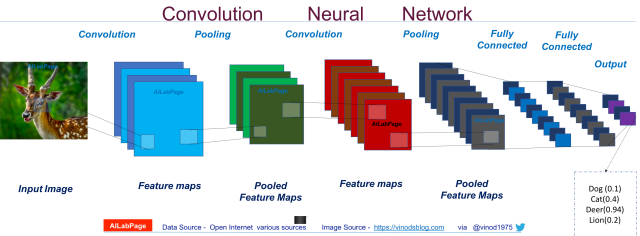
\includegraphics[width=120mm]{figures/cnn.png}
  \caption{Cartoon depicting layers of a CNN}
  \label{cnn}
\end{figure}

Convolutional Layer

The convolutional layer is the cornerstone of a CNN.
It applies a set of filters (or kernels) to the input image to produce feature maps.
Each filter is a small matrix that slides over the input image to compute a dot product.

Given an input image \( I \) of size \( H \times W \) (height \( H \) and width \( W \)) and a filter \( K \) of size \( k_h \times k_w \) (height \( k_h \) and width \( k_w \)), the output feature map \( O \) can be computed using the convolution operation:

\begin{align}
  O(i, j) &= \sum_{m=0}^{k_h-1} \sum_{n=0}^{k_w-1} I(i+m, j+n) \cdot K(m, n) \\
          &= (I * K)(i, j)
\end{align}

where \( * \) denotes the convolution operation.
The dimensions of the output feature map depend on the stride \( s \) and padding \( p \).
If we use zero-padding and stride \( s = 1 \), the dimensions are:

\begin{align}
  H_{out} &= \frac{H - k_h + 2p}{s} + 1 \\
  W_{out} &= \frac{W - k_w + 2p}{s} + 1
\end{align}

Activation Layer 

The Rectified Linear Unit (ReLU) is one of the most commonly used activation functions in CNNs.

This activation function helps in mitigating the vanishing gradient problem and speeds up training.

Pooling Layer

The pooling layer reduces the spatial dimensions of the feature map, which helps in reducing computational complexity and preventing overfitting.
The most common pooling operation is max pooling.
For a pooling window of size \( p_h \times p_w \) and stride \( s \), the max pooling operation is defined as:

\begin{align}
  O_{pool}(i, j) &= \max_{m \in [i:i+p_h], n \in [j:j+p_w]} O_{ReLU}(m, n)
\end{align}

where \( O_{ReLU} \) is the feature map after applying the ReLU activation.
Pooling reduces the dimensions of the feature map:

\begin{align}
  H_{out} &= \frac{H - p_h}{s} + 1 \\
  W_{out} &= \frac{W - p_w}{s} + 1
\end{align}

Fully Connected Layer

The fully connected layer (FC layer) is typically used at the end of the network to produce the final classification results.
It connects every neuron in the previous layer to every neuron in the current layer.
The output of a fully connected layer is computed as:

\begin{align}
  z_j &= \sum_{i=1}^{N} w_{ij} x_i + b_j
\end{align}

where \( w_{ij} \) are the weights, \( x_i \) are the inputs from the previous layer, and \( b_j \) is the bias.
This results in a vector of size equal to the number of classes, which can be fed into a softmax function for classification:

\begin{align}
  \text{Softmax}(z_j) &= \frac{e^{z_j}}{\sum_{k} e^{z_k}}
\end{align}

These layers work together to learn hierarchical features from raw data, making CNNs highly effective for various image processing tasks.



\subsection{Graph Neural Networks}

Graph Neural Networks (GNNs) extend neural network methodologies to handle data represented in the form of graphs.
GNNs are designed to work with the complex, non-Euclidean structure of graphs.
Graphs consist of nodes (or vertices) and edges (connections between nodes), and GNNs leverage these structures to learn representations of nodes and their relationships\cite{Scarselli_Gori_Tsoi_Hagenbuchner_Monfardini_2009}.

To understand how GNNs function, it's important to break down their key components: node features, edge features, and the message-passing mechanism.

In a graph, each node can have associated features, which are typically represented as vectors.
If we denote the feature vector of node \( v \) as \( \mathbf{h}_v \), then the node features for all nodes in the graph can be organized into a matrix \( \mathbf{H} \), where each row corresponds to a node's feature vector.

Similarly, edges in a graph can also have features.
For an edge connecting nodes \( u \) and \( v \), we denote the edge features as \( \mathbf{e}_{uv} \).
These features can be organized into an edge feature matrix \( \mathbf{E} \) \cite{Wu_Cui_Pei_Zhao_2022}.

The core idea of GNNs is the message-passing mechanism, which allows nodes to aggregate information from their neighbors.
This process involves the following steps:

\begin{enumerate}

\item Message Computation:
  For each node \( v \), we compute messages from its neighboring nodes \( \mathcal{N}(v) \).
  The message \( m_{uv} \) from node \( u \) to node \( v \) is typically computed using a function \( \phi \), which can depend on the features of both nodes and the edge between them:

  \begin{align}
    m_{uv} &= \phi(\mathbf{h}_u, \mathbf{h}_v, \mathbf{e}_{uv}) \\
           &= \phi(\mathbf{h}_u, \mathbf{e}_{uv})
  \end{align}

\item Aggregation:
  After computing the messages, each node aggregates the messages from its neighbors.
  The aggregation function \( \text{AGG} \) could be a sum, mean, or a more complex operation:

  \begin{align}
    \mathbf{m}_v &= \text{AGG}_{u \in \mathcal{N}(v)} m_{uv}
  \end{align}

\item Update:
  The aggregated message is then used to update the node’s feature vector.
  This update function \( \text{UPDATE} \) often involves a neural network layer like a fully connected layer or a more complex function:

  \begin{align}
    \mathbf{h}_v' &= \text{UPDATE}(\mathbf{h}_v, \mathbf{m}_v)
  \end{align}

  The updated feature vector \( \mathbf{h}_v' \) represents the new state of the node after considering its neighbors.

  Different GNN architectures can use various choices for the aggregation and update functions \cite{Micheli_2009}.

\end{enumerate}

Graph Neural Networks allow for the processing of graph-structured data by iteratively updating node features through message passing.
This approach allows GNNs to capture complex relationships between nodes and learn meaningful representations that are useful for various tasks such as node classification and graph classification.

\subsection{Model Development}

Developing a neural net isn't just about figuring out the neurons for the network and adjusting the weights.
The task of making a neural net can be broken up into 3 main parts.

\begin{figure}[H]
\centering
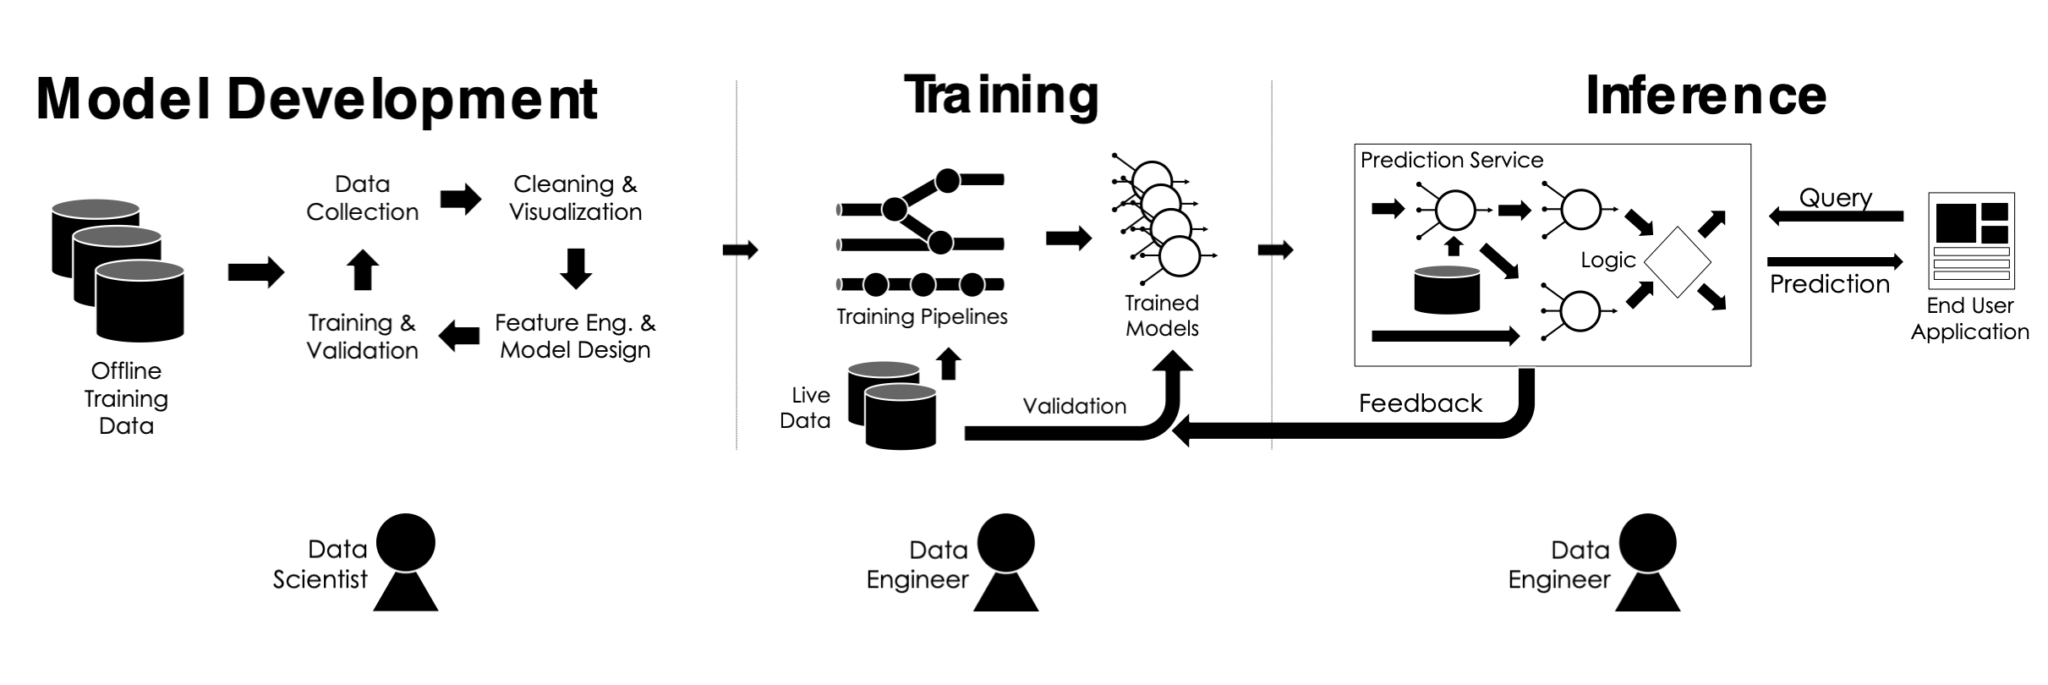
\includegraphics[width=120mm]{figures/mlLifecycle.png}
\caption{Model development}
\label{lifecycle}
\end{figure}

The first step of any kind of model development is looking at both what kind of data is available as well as what kind of input we might want to make on the model.
The data may be scattered about in many places and often will require processing before it can be vectorized.

In the context of neutrino reconstruction, this may require running monte carlo simulations with standard software e.g. (LArSoft, NDsim) and then taking the output from those simulations, processing it into standard images that libraries like pytorch or tensorflow can take as input.
It is also important to think about standardizing the size of those images and thinking about how to toss out the sheer amount of data that has no hits in it because neutrino events are so sparse.

Once that has been done, we can look at actually implementing a neural network based on that data.
This involves setting out training pipelines which will determine how the data flows, as well as figuring out the structure of the network that will be made.
Tests also have to be written for the network so that it can be deployed robustly.
Once the training with the training dataset is complete, the model has to be validated with a validation dataset.
The validation set will also be a set where the answers are previously known so we can see how well the model performs on data that it hasn't previously been run on.

Once the model has been validated, it can finally be deployed for real world data where we don't have the answers.
This is the inference part of the model lifecycle.



\subsection{Model Optimization}

There are two parts where a model can be optimized.
The first is the training phase.
Models can take a long time to train even if a lot of data is available which means it is often worth it to optimize the training phase.
This sort of optimization is called hyperparameter optimization because the actual hyperparameters (weights and biases) aren't being tweaked but rather the parameters that guide how they are formed.
It involves manipulating the structure of the network as well as changing factors such as the learning rate.
The difference between a naive implementation and an optimized one may lead to a speedup of hours for the training.

Training isn't however what a network is spending most of its time doing.
Most of the time a network is used to query for answers, i.e.\ inference.
Inference speedups can be done through a number of ways such as using more specialized hardware like FPGA's or working with TensorRT optimization.
That can bring down the time it takes to query the model for information which can vastly affect number of events being processed in any time period thus increasing throughput.










 